\documentclass[]{article}
\usepackage{lmodern}
\usepackage{amssymb,amsmath}
\usepackage{ifxetex,ifluatex}
\usepackage{fixltx2e} % provides \textsubscript
\ifnum 0\ifxetex 1\fi\ifluatex 1\fi=0 % if pdftex
  \usepackage[T1]{fontenc}
  \usepackage[utf8]{inputenc}
\else % if luatex or xelatex
  \ifxetex
    \usepackage{mathspec}
  \else
    \usepackage{fontspec}
  \fi
  \defaultfontfeatures{Ligatures=TeX,Scale=MatchLowercase}
\fi
% use upquote if available, for straight quotes in verbatim environments
\IfFileExists{upquote.sty}{\usepackage{upquote}}{}
% use microtype if available
\IfFileExists{microtype.sty}{%
\usepackage{microtype}
\UseMicrotypeSet[protrusion]{basicmath} % disable protrusion for tt fonts
}{}
\usepackage{hyperref}
\hypersetup{unicode=true,
            pdftitle={Arranging logger data from HoboLink},
            pdfauthor={Jens Åström},
            pdfborder={0 0 0},
            breaklinks=true}
\urlstyle{same}  % don't use monospace font for urls
\usepackage{color}
\usepackage{fancyvrb}
\newcommand{\VerbBar}{|}
\newcommand{\VERB}{\Verb[commandchars=\\\{\}]}
\DefineVerbatimEnvironment{Highlighting}{Verbatim}{commandchars=\\\{\}}
% Add ',fontsize=\small' for more characters per line
\usepackage{framed}
\definecolor{shadecolor}{RGB}{248,248,248}
\newenvironment{Shaded}{\begin{snugshade}}{\end{snugshade}}
\newcommand{\AlertTok}[1]{\textcolor[rgb]{0.94,0.16,0.16}{#1}}
\newcommand{\AnnotationTok}[1]{\textcolor[rgb]{0.56,0.35,0.01}{\textbf{\textit{#1}}}}
\newcommand{\AttributeTok}[1]{\textcolor[rgb]{0.77,0.63,0.00}{#1}}
\newcommand{\BaseNTok}[1]{\textcolor[rgb]{0.00,0.00,0.81}{#1}}
\newcommand{\BuiltInTok}[1]{#1}
\newcommand{\CharTok}[1]{\textcolor[rgb]{0.31,0.60,0.02}{#1}}
\newcommand{\CommentTok}[1]{\textcolor[rgb]{0.56,0.35,0.01}{\textit{#1}}}
\newcommand{\CommentVarTok}[1]{\textcolor[rgb]{0.56,0.35,0.01}{\textbf{\textit{#1}}}}
\newcommand{\ConstantTok}[1]{\textcolor[rgb]{0.00,0.00,0.00}{#1}}
\newcommand{\ControlFlowTok}[1]{\textcolor[rgb]{0.13,0.29,0.53}{\textbf{#1}}}
\newcommand{\DataTypeTok}[1]{\textcolor[rgb]{0.13,0.29,0.53}{#1}}
\newcommand{\DecValTok}[1]{\textcolor[rgb]{0.00,0.00,0.81}{#1}}
\newcommand{\DocumentationTok}[1]{\textcolor[rgb]{0.56,0.35,0.01}{\textbf{\textit{#1}}}}
\newcommand{\ErrorTok}[1]{\textcolor[rgb]{0.64,0.00,0.00}{\textbf{#1}}}
\newcommand{\ExtensionTok}[1]{#1}
\newcommand{\FloatTok}[1]{\textcolor[rgb]{0.00,0.00,0.81}{#1}}
\newcommand{\FunctionTok}[1]{\textcolor[rgb]{0.00,0.00,0.00}{#1}}
\newcommand{\ImportTok}[1]{#1}
\newcommand{\InformationTok}[1]{\textcolor[rgb]{0.56,0.35,0.01}{\textbf{\textit{#1}}}}
\newcommand{\KeywordTok}[1]{\textcolor[rgb]{0.13,0.29,0.53}{\textbf{#1}}}
\newcommand{\NormalTok}[1]{#1}
\newcommand{\OperatorTok}[1]{\textcolor[rgb]{0.81,0.36,0.00}{\textbf{#1}}}
\newcommand{\OtherTok}[1]{\textcolor[rgb]{0.56,0.35,0.01}{#1}}
\newcommand{\PreprocessorTok}[1]{\textcolor[rgb]{0.56,0.35,0.01}{\textit{#1}}}
\newcommand{\RegionMarkerTok}[1]{#1}
\newcommand{\SpecialCharTok}[1]{\textcolor[rgb]{0.00,0.00,0.00}{#1}}
\newcommand{\SpecialStringTok}[1]{\textcolor[rgb]{0.31,0.60,0.02}{#1}}
\newcommand{\StringTok}[1]{\textcolor[rgb]{0.31,0.60,0.02}{#1}}
\newcommand{\VariableTok}[1]{\textcolor[rgb]{0.00,0.00,0.00}{#1}}
\newcommand{\VerbatimStringTok}[1]{\textcolor[rgb]{0.31,0.60,0.02}{#1}}
\newcommand{\WarningTok}[1]{\textcolor[rgb]{0.56,0.35,0.01}{\textbf{\textit{#1}}}}
\usepackage{graphicx,grffile}
\makeatletter
\def\maxwidth{\ifdim\Gin@nat@width>\linewidth\linewidth\else\Gin@nat@width\fi}
\def\maxheight{\ifdim\Gin@nat@height>\textheight\textheight\else\Gin@nat@height\fi}
\makeatother
% Scale images if necessary, so that they will not overflow the page
% margins by default, and it is still possible to overwrite the defaults
% using explicit options in \includegraphics[width, height, ...]{}
\setkeys{Gin}{width=\maxwidth,height=\maxheight,keepaspectratio}
\IfFileExists{parskip.sty}{%
\usepackage{parskip}
}{% else
\setlength{\parindent}{0pt}
\setlength{\parskip}{6pt plus 2pt minus 1pt}
}
\setlength{\emergencystretch}{3em}  % prevent overfull lines
\providecommand{\tightlist}{%
  \setlength{\itemsep}{0pt}\setlength{\parskip}{0pt}}
\setcounter{secnumdepth}{0}
% Redefines (sub)paragraphs to behave more like sections
\ifx\paragraph\undefined\else
\let\oldparagraph\paragraph
\renewcommand{\paragraph}[1]{\oldparagraph{#1}\mbox{}}
\fi
\ifx\subparagraph\undefined\else
\let\oldsubparagraph\subparagraph
\renewcommand{\subparagraph}[1]{\oldsubparagraph{#1}\mbox{}}
\fi

%%% Use protect on footnotes to avoid problems with footnotes in titles
\let\rmarkdownfootnote\footnote%
\def\footnote{\protect\rmarkdownfootnote}

%%% Change title format to be more compact
\usepackage{titling}

% Create subtitle command for use in maketitle
\newcommand{\subtitle}[1]{
  \posttitle{
    \begin{center}\large#1\end{center}
    }
}

\setlength{\droptitle}{-2em}
  \title{Arranging logger data from HoboLink}
  \pretitle{\vspace{\droptitle}\centering\huge}
  \posttitle{\par}
  \author{Jens Åström}
  \preauthor{\centering\large\emph}
  \postauthor{\par}
  \predate{\centering\large\emph}
  \postdate{\par}
  \date{26 June, 2020}


%\linespread{1.3}


% You know, for landscape
\usepackage{lscape}
\usepackage{pdfpages}


% pandoc does not parse latex env - https://groups.google.com/forum/?fromgroups=#!topic/pandoc-discuss/oZETB5Ii1Cw
\newcommand{\blandscape}{\begin{landscape}}
\newcommand{\elandscape}{\end{landscape}}

% Make new page before each section
%\let\stdsection\section
%\renewcommand\section{\newpage\stdsection}

% Highlight inline `code`
\usepackage{soul}
\usepackage{xcolor}

\definecolor{Light}{gray}{.97}
\sethlcolor{Light}

\let\OldTexttt\texttt
\renewcommand{\texttt}[1]{\OldTexttt{\hl{#1}}}


\clubpenalty=10000      %kara za sierotki
\widowpenalty=10000  % nie pozostawiaj wdów
\brokenpenalty=10000    % nie dziel wyrazów miêdzy stronami
\exhyphenpenalty=999999   % nie dziel s³ów z myœlnikiem
\righthyphenmin=3     % dziel minimum 3 litery

\renewcommand{\topfraction}{0.95}
\renewcommand{\bottomfraction}{0.95}
\renewcommand{\textfraction}{0.05}
\renewcommand{\floatpagefraction}{0.35}

\begin{document}
\maketitle

{
\setcounter{tocdepth}{2}
\tableofcontents
}
\hypertarget{intro}{%
\section{Intro}\label{intro}}

The data exports for the temperature and humidity MX loggers from Hobo
needs a bit of data wrangling before it can be used. The different data
streams from each logger all get a separate column. Here we develop a
script to turn this into a more usable long format.

\hypertarget{read-in-data}{%
\section{Read in data}\label{read-in-data}}

I have a single export with many loggers, as a csv file.

\begin{Shaded}
\begin{Highlighting}[]
\NormalTok{inputFile <{-}}\StringTok{ "../rawData/All\_MX\_2020\_2020\_06\_26\_09\_20\_43\_UTC\_1.csv"}

\NormalTok{rawDat <{-}}\StringTok{ }\KeywordTok{read\_csv}\NormalTok{(inputFile,}\DataTypeTok{col\_types =} \KeywordTok{cols}\NormalTok{(}\DataTypeTok{.default =} \StringTok{"c"}\NormalTok{))}

\NormalTok{dat <{-}}\StringTok{ }\NormalTok{rawDat }\OperatorTok{\%>\%}\StringTok{  }
\StringTok{  }\KeywordTok{select}\NormalTok{(}\OperatorTok{{-}}\StringTok{"Line\#"}\NormalTok{) }\OperatorTok{\%>\%}\StringTok{ }
\StringTok{  }\KeywordTok{mutate}\NormalTok{(}\DataTypeTok{date =} \KeywordTok{as.POSIXct}\NormalTok{(Date, }\DataTypeTok{format =} \StringTok{"\%m/\%d/\%y \%H:\%M:\%S"}\NormalTok{)) }\OperatorTok{\%>\%}\StringTok{ }
\StringTok{  }\KeywordTok{mutate\_if}\NormalTok{(is\_character, as.double) }\OperatorTok{\%>\%}\StringTok{ }
\StringTok{  }\KeywordTok{select}\NormalTok{(}\OperatorTok{{-}}\NormalTok{Date)}
\end{Highlighting}
\end{Shaded}

\begin{verbatim}
## Warning: NAs introduced by coercion
\end{verbatim}

\begin{Shaded}
\begin{Highlighting}[]
\NormalTok{dat}
\end{Highlighting}
\end{Shaded}

\begin{verbatim}
## # A tibble: 6,889 x 64
##    `Temperature (M~ `RH (MX-RH-2 20~ `Dew Point (MX-~ `Temperature (M~
##               <dbl>            <dbl>            <dbl>            <dbl>
##  1             NA               NA              NA                  NA
##  2             NA               NA              NA                  NA
##  3             22.3             28.2             3.05               NA
##  4             NA               NA              NA                  NA
##  5             24.7             25.6             3.69               NA
##  6             NA               NA              NA                  NA
##  7             25.5             24.4             3.72               NA
##  8             NA               NA              NA                  NA
##  9             26.1             24.0             3.95               NA
## 10             NA               NA              NA                  NA
## # ... with 6,879 more rows, and 60 more variables: `RH (MX-RH-2
## #   20835815:20835815-2), %, 20835815` <dbl>, `Dew Point (MX-TEMP-2
## #   20835815:20835815-4), *C, 20835815` <dbl>, `Temperature (MX-TEMP-2
## #   20835816:20835816-1), *C, 20835816` <dbl>, `RH (MX-RH-2
## #   20835816:20835816-2), %, 20835816` <dbl>, `Dew Point (MX-TEMP-2
## #   20835816:20835816-4), *C, 20835816` <dbl>, `Temperature (MX-TEMP-2
## #   20835817:20835817-1), *C, 20835817` <dbl>, `RH (MX-RH-2
## #   20835817:20835817-2), %, 20835817` <dbl>, `Dew Point (MX-TEMP-2
## #   20835817:20835817-4), *C, 20835817` <dbl>, `Temperature (MX-TEMP-2
## #   20835818:20835818-1), *C, 20835818` <dbl>, `RH (MX-RH-2
## #   20835818:20835818-2), %, 20835818` <dbl>, `Dew Point (MX-TEMP-2
## #   20835818:20835818-4), *C, 20835818` <dbl>, `Temperature (MX-TEMP-2
## #   20835819:20835819-1), *C, 20835819` <dbl>, `RH (MX-RH-2
## #   20835819:20835819-2), %, 20835819` <dbl>, `Dew Point (MX-TEMP-2
## #   20835819:20835819-4), *C, 20835819` <dbl>, `Temperature (MX-TEMP-2
## #   20835820:20835820-1), *C, 20835820` <dbl>, `RH (MX-RH-2
## #   20835820:20835820-2), %, 20835820` <dbl>, `Dew Point (MX-TEMP-2
## #   20835820:20835820-4), *C, 20835820` <dbl>, `Temperature (MX-TEMP-2
## #   20835821:20835821-1), *C, 20835821` <dbl>, `RH (MX-RH-2
## #   20835821:20835821-2), %, 20835821` <dbl>, `Dew Point (MX-TEMP-2
## #   20835821:20835821-4), *C, 20835821` <dbl>, `Temperature (MX-TEMP-2
## #   20835822:20835822-1), *C, 20835822` <dbl>, `RH (MX-RH-2
## #   20835822:20835822-2), %, 20835822` <dbl>, `Dew Point (MX-TEMP-2
## #   20835822:20835822-4), *C, 20835822` <dbl>, `Temperature (MX-TEMP-2
## #   20835823:20835823-1), *C, 20835823` <dbl>, `RH (MX-RH-2
## #   20835823:20835823-2), %, 20835823` <dbl>, `Dew Point (MX-TEMP-2
## #   20835823:20835823-4), *C, 20835823` <dbl>, `Temperature (MX-TEMP-2
## #   20835824:20835824-1), *C, 20835824` <dbl>, `RH (MX-RH-2
## #   20835824:20835824-2), %, 20835824` <dbl>, `Dew Point (MX-TEMP-2
## #   20835824:20835824-4), *C, 20835824` <dbl>, `Temperature (MX-TEMP-2
## #   20835825:20835825-1), *C, 20835825` <dbl>, `RH (MX-RH-2
## #   20835825:20835825-2), %, 20835825` <dbl>, `Dew Point (MX-TEMP-2
## #   20835825:20835825-4), *C, 20835825` <dbl>, `Temperature (MX-TEMP-2
## #   20843228:20843228-1), *C, 20843228` <dbl>, `RH (MX-RH-2
## #   20843228:20843228-2), %, 20843228` <dbl>, `Dew Point (MX-TEMP-2
## #   20843228:20843228-4), *C, 20843228` <dbl>, `Temperature (MX-TEMP-2
## #   20843229:20843229-1), *C, 20843229` <dbl>, `RH (MX-RH-2
## #   20843229:20843229-2), %, 20843229` <dbl>, `Dew Point (MX-TEMP-2
## #   20843229:20843229-4), *C, 20843229` <dbl>, `Temperature (MX-TEMP-2
## #   20843230:20843230-1), *C, 20843230` <dbl>, `RH (MX-RH-2
## #   20843230:20843230-2), %, 20843230` <dbl>, `Dew Point (MX-TEMP-2
## #   20843230:20843230-4), *C, 20843230` <dbl>, `Temperature (MX-TEMP-2
## #   20843231:20843231-1), *C, 20843231` <dbl>, `RH (MX-RH-2
## #   20843231:20843231-2), %, 20843231` <dbl>, `Dew Point (MX-TEMP-2
## #   20843231:20843231-4), *C, 20843231` <dbl>, `Temperature (MX-TEMP-2
## #   20843233:20843233-1), *C, 20843233` <dbl>, `RH (MX-RH-2
## #   20843233:20843233-2), %, 20843233` <dbl>, `Dew Point (MX-TEMP-2
## #   20843233:20843233-4), *C, 20843233` <dbl>, `Temperature (MX-TEMP-2
## #   20843235:20843235-1), *C, 20843235` <dbl>, `RH (MX-RH-2
## #   20843235:20843235-2), %, 20843235` <dbl>, `Dew Point (MX-TEMP-2
## #   20843235:20843235-4), *C, 20843235` <dbl>, `Temperature (MX-TEMP-2
## #   20843236:20843236-1), *C, 20843236` <dbl>, `RH (MX-RH-2
## #   20843236:20843236-2), %, 20843236` <dbl>, `Dew Point (MX-TEMP-2
## #   20843236:20843236-4), *C, 20843236` <dbl>, `Temperature (MX-TEMP-2
## #   20843238:20843238-1), *C, 20843238` <dbl>, `RH (MX-RH-2
## #   20843238:20843238-2), %, 20843238` <dbl>, `Dew Point (MX-TEMP-2
## #   20843238:20843238-4), *C, 20843238` <dbl>, `Temperature (MX-TEMP-2
## #   20843239:20843239-1), *C, 20843239` <dbl>, `RH (MX-RH-2
## #   20843239:20843239-2), %, 20843239` <dbl>, `Dew Point (MX-TEMP-2
## #   20843239:20843239-4), *C, 20843239` <dbl>, date <dttm>
\end{verbatim}

That's quite the number of columns\ldots{}

We have to pivot this data set to a longer format. We also get rid of
the rows with no data.

\begin{Shaded}
\begin{Highlighting}[]
\NormalTok{temp <{-}}\StringTok{ }\NormalTok{dat }\OperatorTok{\%>\%}\StringTok{ }
\StringTok{  }\KeywordTok{pivot\_longer}\NormalTok{(}\DataTypeTok{cols =} \KeywordTok{starts\_with}\NormalTok{(}\StringTok{"Temperature"}\NormalTok{),}
               \DataTypeTok{names\_to =} \StringTok{"logger"}\NormalTok{,}
               \DataTypeTok{values\_to =} \StringTok{"temperature"}\NormalTok{) }\OperatorTok{\%>\%}\StringTok{ }
\StringTok{  }\KeywordTok{select}\NormalTok{(date,}
\NormalTok{         logger,}
\NormalTok{         temperature) }\OperatorTok{\%>\%}\StringTok{ }
\StringTok{  }\KeywordTok{filter}\NormalTok{(}\OperatorTok{!}\KeywordTok{is.na}\NormalTok{(temperature))}

\NormalTok{rh <{-}}\StringTok{ }\NormalTok{dat }\OperatorTok{\%>\%}\StringTok{ }
\StringTok{  }\KeywordTok{pivot\_longer}\NormalTok{(}\DataTypeTok{cols =} \KeywordTok{starts\_with}\NormalTok{(}\StringTok{"RH"}\NormalTok{),}
               \DataTypeTok{names\_to =} \StringTok{"logger"}\NormalTok{,}
               \DataTypeTok{values\_to =} \StringTok{"rh"}\NormalTok{) }\OperatorTok{\%>\%}\StringTok{ }
\StringTok{  }\KeywordTok{select}\NormalTok{(date,}
\NormalTok{         logger,}
\NormalTok{         rh)}\OperatorTok{\%>\%}\StringTok{ }
\StringTok{  }\KeywordTok{filter}\NormalTok{(}\OperatorTok{!}\KeywordTok{is.na}\NormalTok{(rh))}

\NormalTok{dew  <{-}}\StringTok{ }\NormalTok{dat }\OperatorTok{\%>\%}\StringTok{ }
\StringTok{  }\KeywordTok{pivot\_longer}\NormalTok{(}\DataTypeTok{cols =} \KeywordTok{starts\_with}\NormalTok{(}\StringTok{"Dew"}\NormalTok{),}
               \DataTypeTok{names\_to =} \StringTok{"logger"}\NormalTok{,}
               \DataTypeTok{values\_to =} \StringTok{"dew"}\NormalTok{) }\OperatorTok{\%>\%}\StringTok{ }
\StringTok{  }\KeywordTok{select}\NormalTok{(date,}
\NormalTok{         logger,}
\NormalTok{         dew) }\OperatorTok{\%>\%}\StringTok{ }
\StringTok{  }\KeywordTok{filter}\NormalTok{(}\OperatorTok{!}\KeywordTok{is.na}\NormalTok{(dew))}
\end{Highlighting}
\end{Shaded}

The data now looks like this

\begin{Shaded}
\begin{Highlighting}[]
\NormalTok{temp}
\end{Highlighting}
\end{Shaded}

\begin{verbatim}
## # A tibble: 6,889 x 3
##    date                logger                                   temperature
##    <dttm>              <chr>                                          <dbl>
##  1 2020-05-14 08:21:51 Temperature (MX-TEMP-2 20843236:2084323~        20.8
##  2 2020-05-14 08:41:51 Temperature (MX-TEMP-2 20843236:2084323~        22.2
##  3 2020-05-14 08:54:29 Temperature (MX-TEMP-2 20835814:2083581~        22.3
##  4 2020-05-14 09:01:51 Temperature (MX-TEMP-2 20843236:2084323~        24.9
##  5 2020-05-14 09:14:29 Temperature (MX-TEMP-2 20835814:2083581~        24.7
##  6 2020-05-14 09:21:51 Temperature (MX-TEMP-2 20843236:2084323~        26.2
##  7 2020-05-14 09:34:29 Temperature (MX-TEMP-2 20835814:2083581~        25.5
##  8 2020-05-14 09:41:51 Temperature (MX-TEMP-2 20843236:2084323~        26.6
##  9 2020-05-14 09:54:29 Temperature (MX-TEMP-2 20835814:2083581~        26.1
## 10 2020-05-14 10:01:51 Temperature (MX-TEMP-2 20843236:2084323~        27.2
## # ... with 6,879 more rows
\end{verbatim}

Time to strip the logger names and merge the tables

\begin{Shaded}
\begin{Highlighting}[]
\NormalTok{temp <{-}}\StringTok{ }\NormalTok{temp }\OperatorTok{\%>\%}\StringTok{ }
\StringTok{  }\KeywordTok{mutate}\NormalTok{(}\DataTypeTok{logger =} \KeywordTok{str\_extract}\NormalTok{(logger,}
                              \StringTok{"[\^{}, ]+$"}\NormalTok{))}

\NormalTok{rh <{-}}\StringTok{ }\NormalTok{rh }\OperatorTok{\%>\%}\StringTok{ }
\StringTok{  }\KeywordTok{mutate}\NormalTok{(}\DataTypeTok{logger =} \KeywordTok{str\_extract}\NormalTok{(logger,}
                              \StringTok{"[\^{}, ]+$"}\NormalTok{))}
\NormalTok{dew <{-}}\StringTok{ }\NormalTok{dew }\OperatorTok{\%>\%}\StringTok{ }
\StringTok{  }\KeywordTok{mutate}\NormalTok{(}\DataTypeTok{logger =} \KeywordTok{str\_extract}\NormalTok{(logger,}
                              \StringTok{"[\^{}, ]+$"}\NormalTok{))}
\end{Highlighting}
\end{Shaded}

Check to see that the dates are the same for the datasets

\begin{Shaded}
\begin{Highlighting}[]
\KeywordTok{all}\NormalTok{(}\KeywordTok{all}\NormalTok{(temp}\OperatorTok{$}\NormalTok{date }\OperatorTok{==}\StringTok{ }\NormalTok{rh}\OperatorTok{$}\NormalTok{date),}
\KeywordTok{all}\NormalTok{(rh}\OperatorTok{$}\NormalTok{date }\OperatorTok{==}\StringTok{ }\NormalTok{dew}\OperatorTok{$}\NormalTok{date))}
\end{Highlighting}
\end{Shaded}

\begin{verbatim}
## [1] TRUE
\end{verbatim}

\begin{Shaded}
\begin{Highlighting}[]
\NormalTok{combDat <{-}}\StringTok{ }\NormalTok{temp }\OperatorTok{\%>\%}\StringTok{ }
\StringTok{  }\KeywordTok{full\_join}\NormalTok{(rh,}
             \DataTypeTok{by =} \KeywordTok{c}\NormalTok{(}\StringTok{"date"}\NormalTok{ =}\StringTok{ "date"}\NormalTok{,}
                    \StringTok{"logger"}\NormalTok{ =}\StringTok{ "logger"}\NormalTok{)) }\OperatorTok{\%>\%}\StringTok{ }
\StringTok{  }\KeywordTok{full\_join}\NormalTok{(dew,}
            \DataTypeTok{by =} \KeywordTok{c}\NormalTok{(}\StringTok{"date"}\NormalTok{ =}\StringTok{ "date"}\NormalTok{,}
                    \StringTok{"logger"}\NormalTok{ =}\StringTok{ "logger"}\NormalTok{)) }\OperatorTok{\%>\%}\StringTok{ }
\StringTok{  }\KeywordTok{arrange}\NormalTok{(logger,}
\NormalTok{          date)}
\end{Highlighting}
\end{Shaded}

\begin{Shaded}
\begin{Highlighting}[]
\NormalTok{combDat}
\end{Highlighting}
\end{Shaded}

\begin{verbatim}
## # A tibble: 6,889 x 5
##    date                logger   temperature    rh   dew
##    <dttm>              <chr>          <dbl> <dbl> <dbl>
##  1 2020-05-14 08:54:29 20835814       22.3   28.2  3.05
##  2 2020-05-14 09:14:29 20835814       24.7   25.6  3.69
##  3 2020-05-14 09:34:29 20835814       25.5   24.4  3.72
##  4 2020-05-14 09:54:29 20835814       26.1   24.0  3.95
##  5 2020-05-14 10:14:29 20835814       26.5   23.2  3.83
##  6 2020-05-14 10:34:29 20835814       26.5   23.3  3.91
##  7 2020-05-14 10:54:29 20835814       20.6   19.5 -3.47
##  8 2020-05-14 11:14:29 20835814        5.32  47.9 -4.83
##  9 2020-05-14 11:34:29 20835814        4.53  53.3 -4.13
## 10 2020-05-14 14:39:05 20835814        1.88  79.3 -1.32
## # ... with 6,879 more rows
\end{verbatim}

\hypertarget{package-this-into-a-funtion}{%
\section{Package this into a
funtion}\label{package-this-into-a-funtion}}

\begin{Shaded}
\begin{Highlighting}[]
\NormalTok{longerHobo <{-}}\StringTok{ }\ControlFlowTok{function}\NormalTok{(inputFile)\{}
  
\NormalTok{  rawDat <{-}}\StringTok{ }\KeywordTok{read\_csv}\NormalTok{(inputFile,}\DataTypeTok{col\_types =} \KeywordTok{cols}\NormalTok{(}\DataTypeTok{.default =} \StringTok{"c"}\NormalTok{))}

\NormalTok{  dat <{-}}\StringTok{ }\NormalTok{rawDat }\OperatorTok{\%>\%}\StringTok{  }
\StringTok{    }\KeywordTok{select}\NormalTok{(}\OperatorTok{{-}}\StringTok{"Line\#"}\NormalTok{) }\OperatorTok{\%>\%}\StringTok{ }
\StringTok{    }\KeywordTok{mutate}\NormalTok{(}\DataTypeTok{date =} \KeywordTok{as.POSIXct}\NormalTok{(Date, }\DataTypeTok{format =} \StringTok{"\%m/\%d/\%y \%H:\%M:\%S"}\NormalTok{)) }\OperatorTok{\%>\%}\StringTok{ }
\StringTok{    }\KeywordTok{mutate\_if}\NormalTok{(is\_character, as.double) }\OperatorTok{\%>\%}\StringTok{ }
\StringTok{    }\KeywordTok{select}\NormalTok{(}\OperatorTok{{-}}\NormalTok{Date)}

\NormalTok{    dat <{-}}\StringTok{ }\NormalTok{rawDat }\OperatorTok{\%>\%}\StringTok{  }
\StringTok{  }\KeywordTok{select}\NormalTok{(}\OperatorTok{{-}}\StringTok{"Line\#"}\NormalTok{) }\OperatorTok{\%>\%}\StringTok{ }
\StringTok{  }\KeywordTok{mutate}\NormalTok{(}\DataTypeTok{date =} \KeywordTok{as.POSIXct}\NormalTok{(Date, }\DataTypeTok{format =} \StringTok{"\%m/\%d/\%y \%H:\%M:\%S"}\NormalTok{)) }\OperatorTok{\%>\%}\StringTok{ }
\StringTok{  }\KeywordTok{mutate\_if}\NormalTok{(is\_character, as.double) }\OperatorTok{\%>\%}\StringTok{ }
\StringTok{  }\KeywordTok{select}\NormalTok{(}\OperatorTok{{-}}\NormalTok{Date)}
 
   
\NormalTok{  temp <{-}}\StringTok{ }\NormalTok{dat }\OperatorTok{\%>\%}\StringTok{ }
\StringTok{    }\KeywordTok{pivot\_longer}\NormalTok{(}\DataTypeTok{cols =} \KeywordTok{starts\_with}\NormalTok{(}\StringTok{"Temperature"}\NormalTok{),}
               \DataTypeTok{names\_to =} \StringTok{"logger"}\NormalTok{,}
               \DataTypeTok{values\_to =} \StringTok{"temperature"}\NormalTok{) }\OperatorTok{\%>\%}\StringTok{ }
\StringTok{    }\KeywordTok{select}\NormalTok{(date,}
\NormalTok{         logger,}
\NormalTok{         temperature) }\OperatorTok{\%>\%}\StringTok{ }
\StringTok{    }\KeywordTok{filter}\NormalTok{(}\OperatorTok{!}\KeywordTok{is.na}\NormalTok{(temperature))}

\NormalTok{  rh <{-}}\StringTok{ }\NormalTok{dat }\OperatorTok{\%>\%}\StringTok{ }
\StringTok{    }\KeywordTok{pivot\_longer}\NormalTok{(}\DataTypeTok{cols =} \KeywordTok{starts\_with}\NormalTok{(}\StringTok{"RH"}\NormalTok{),}
                 \DataTypeTok{names\_to =} \StringTok{"logger"}\NormalTok{,}
                 \DataTypeTok{values\_to =} \StringTok{"rh"}\NormalTok{) }\OperatorTok{\%>\%}\StringTok{ }
\StringTok{    }\KeywordTok{select}\NormalTok{(date,}
\NormalTok{           logger,}
\NormalTok{           rh)}\OperatorTok{\%>\%}\StringTok{ }
\StringTok{    }\KeywordTok{filter}\NormalTok{(}\OperatorTok{!}\KeywordTok{is.na}\NormalTok{(rh))}
  
\NormalTok{  dew  <{-}}\StringTok{ }\NormalTok{dat }\OperatorTok{\%>\%}\StringTok{ }
\StringTok{    }\KeywordTok{pivot\_longer}\NormalTok{(}\DataTypeTok{cols =} \KeywordTok{starts\_with}\NormalTok{(}\StringTok{"Dew"}\NormalTok{),}
                 \DataTypeTok{names\_to =} \StringTok{"logger"}\NormalTok{,}
                 \DataTypeTok{values\_to =} \StringTok{"dew"}\NormalTok{) }\OperatorTok{\%>\%}\StringTok{ }
\StringTok{    }\KeywordTok{select}\NormalTok{(date,}
\NormalTok{           logger,}
\NormalTok{           dew) }\OperatorTok{\%>\%}\StringTok{ }
\StringTok{    }\KeywordTok{filter}\NormalTok{(}\OperatorTok{!}\KeywordTok{is.na}\NormalTok{(dew))}
  
  
\NormalTok{  temp <{-}}\StringTok{ }\NormalTok{temp }\OperatorTok{\%>\%}\StringTok{ }
\StringTok{    }\KeywordTok{mutate}\NormalTok{(}\DataTypeTok{logger =} \KeywordTok{str\_extract}\NormalTok{(logger,}
                              \StringTok{"[\^{}, ]+$"}\NormalTok{))}
\NormalTok{  rh <{-}}\StringTok{ }\NormalTok{rh }\OperatorTok{\%>\%}\StringTok{ }
\StringTok{    }\KeywordTok{mutate}\NormalTok{(}\DataTypeTok{logger =} \KeywordTok{str\_extract}\NormalTok{(logger,}
                                \StringTok{"[\^{}, ]+$"}\NormalTok{))}
\NormalTok{  dew <{-}}\StringTok{ }\NormalTok{dew }\OperatorTok{\%>\%}\StringTok{ }
\StringTok{    }\KeywordTok{mutate}\NormalTok{(}\DataTypeTok{logger =} \KeywordTok{str\_extract}\NormalTok{(logger,}
                                \StringTok{"[\^{}, ]+$"}\NormalTok{))}
  
  \ControlFlowTok{if}\NormalTok{(}\OperatorTok{!}\KeywordTok{all}\NormalTok{(}\KeywordTok{all}\NormalTok{(temp}\OperatorTok{$}\NormalTok{date }\OperatorTok{==}\StringTok{ }\NormalTok{rh}\OperatorTok{$}\NormalTok{date),}
  \KeywordTok{all}\NormalTok{(rh}\OperatorTok{$}\NormalTok{date }\OperatorTok{==}\StringTok{ }\NormalTok{dew}\OperatorTok{$}\NormalTok{date))) }\KeywordTok{stop}\NormalTok{(}\StringTok{"Tables datetimes doesn\textquotesingle{}t match"}\NormalTok{)}
  
\NormalTok{  combDat <{-}}\StringTok{ }\NormalTok{temp }\OperatorTok{\%>\%}\StringTok{ }
\StringTok{  }\KeywordTok{full\_join}\NormalTok{(rh,}
             \DataTypeTok{by =} \KeywordTok{c}\NormalTok{(}\StringTok{"date"}\NormalTok{ =}\StringTok{ "date"}\NormalTok{,}
                    \StringTok{"logger"}\NormalTok{ =}\StringTok{ "logger"}\NormalTok{)) }\OperatorTok{\%>\%}\StringTok{ }
\StringTok{  }\KeywordTok{full\_join}\NormalTok{(dew,}
            \DataTypeTok{by =} \KeywordTok{c}\NormalTok{(}\StringTok{"date"}\NormalTok{ =}\StringTok{ "date"}\NormalTok{,}
                    \StringTok{"logger"}\NormalTok{ =}\StringTok{ "logger"}\NormalTok{)) }\OperatorTok{\%>\%}\StringTok{ }
\StringTok{  }\KeywordTok{arrange}\NormalTok{(logger,}
\NormalTok{          date)}
  
  \KeywordTok{return}\NormalTok{(combDat)}
\NormalTok{\}}
\end{Highlighting}
\end{Shaded}

We can check that it produces the same results as the script.

\begin{Shaded}
\begin{Highlighting}[]
\NormalTok{combDat2 <{-}}\StringTok{ }\KeywordTok{longerHobo}\NormalTok{(}\StringTok{"../rawData/All\_MX\_2020\_2020\_06\_26\_09\_20\_43\_UTC\_1.csv"}\NormalTok{)}
\end{Highlighting}
\end{Shaded}

\begin{verbatim}
## Warning: NAs introduced by coercion

## Warning: NAs introduced by coercion
\end{verbatim}

\begin{Shaded}
\begin{Highlighting}[]
\KeywordTok{all}\NormalTok{(combDat }\OperatorTok{==}\StringTok{ }\NormalTok{combDat2)}
\end{Highlighting}
\end{Shaded}

\begin{verbatim}
## [1] TRUE
\end{verbatim}

\hypertarget{check-the-data-out}{%
\section{Check the data out}\label{check-the-data-out}}

\begin{Shaded}
\begin{Highlighting}[]
\KeywordTok{ggplot}\NormalTok{(combDat) }\OperatorTok{+}
\StringTok{  }\KeywordTok{geom\_line}\NormalTok{(}\KeywordTok{aes}\NormalTok{(}\DataTypeTok{x =}\NormalTok{ date, }\DataTypeTok{y =}\NormalTok{ temperature, }\DataTypeTok{color =}\NormalTok{ logger)) }\OperatorTok{+}
\StringTok{  }\KeywordTok{ggtitle}\NormalTok{(}\StringTok{"All the temperatures so far"}\NormalTok{)}
\end{Highlighting}
\end{Shaded}

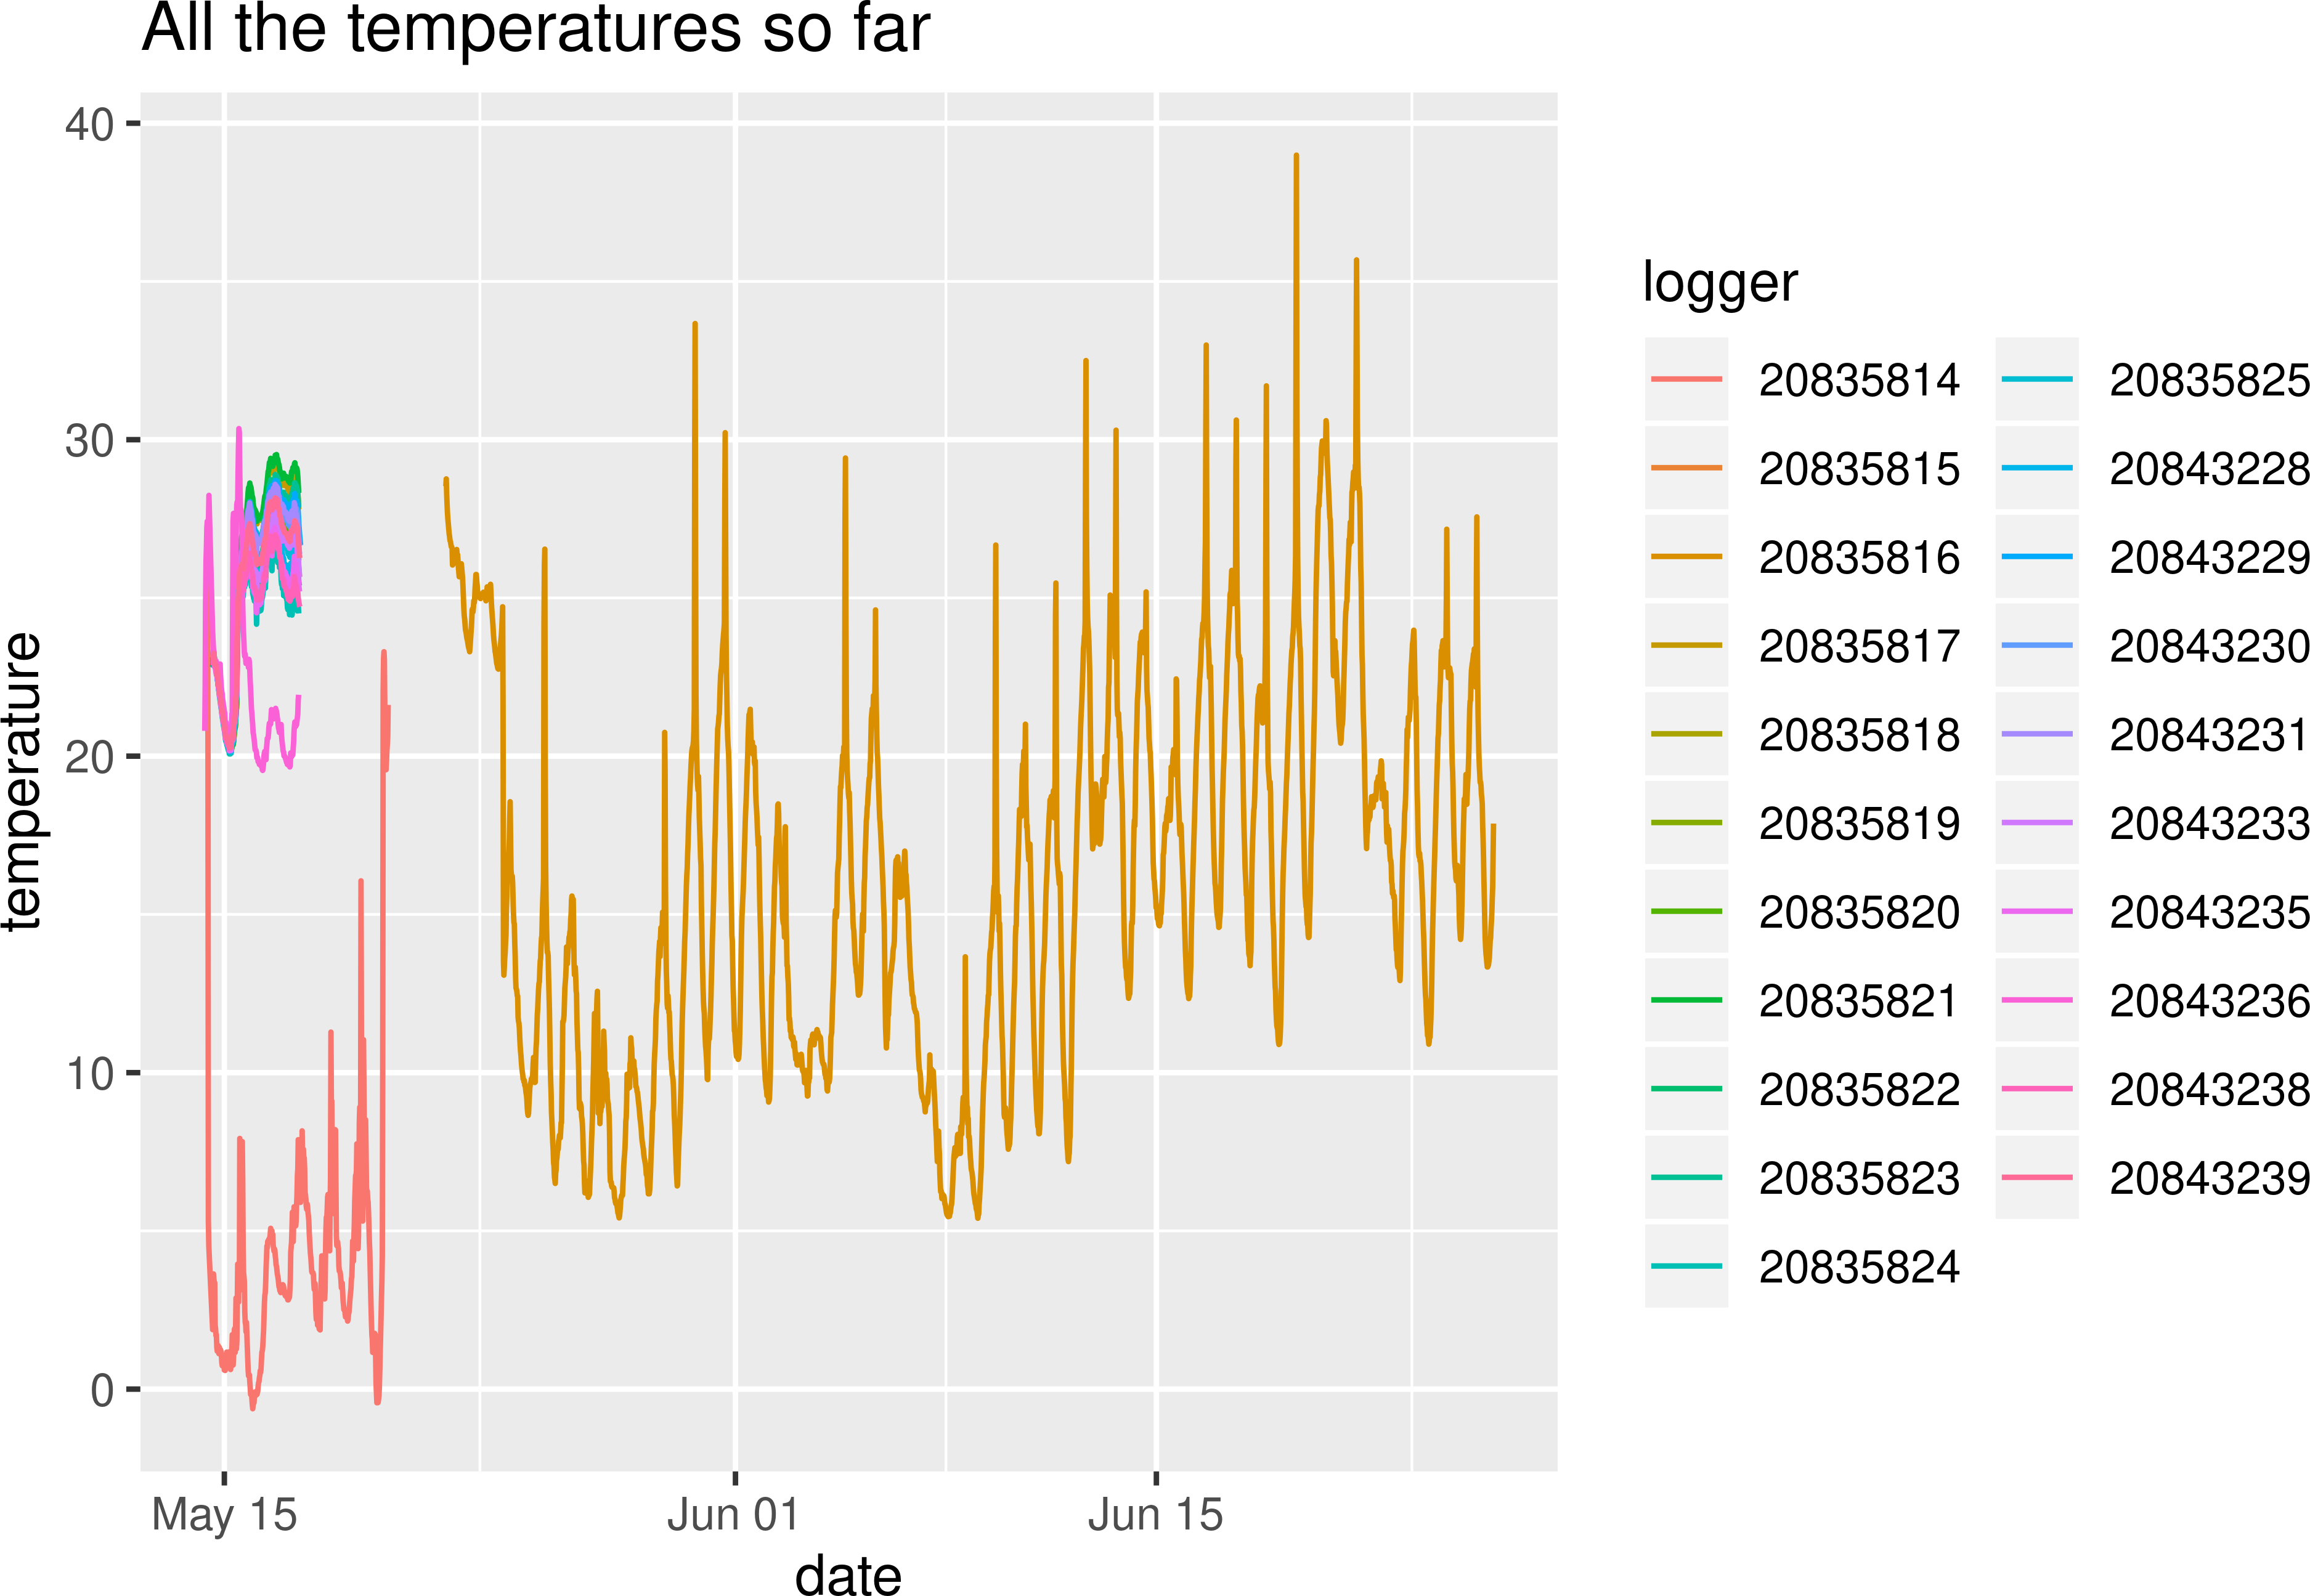
\includegraphics{figure/unnamed-chunk-12-1.png}

\begin{Shaded}
\begin{Highlighting}[]
\NormalTok{oneLogger <{-}}\StringTok{ }\NormalTok{combDat }\OperatorTok{\%>\%}\StringTok{ }
\StringTok{  }\KeywordTok{filter}\NormalTok{(logger }\OperatorTok{==}\StringTok{ "20835816"}\NormalTok{) }\OperatorTok{\%>\%}\StringTok{ }
\StringTok{  }\KeywordTok{select}\NormalTok{(}\DataTypeTok{Date =}\NormalTok{ date, }
\NormalTok{         logger,}
         \DataTypeTok{Temperature =}\NormalTok{ temperature,}
         \DataTypeTok{Relative\_humidity =}\NormalTok{ rh,}
         \DataTypeTok{Dew\_point =}\NormalTok{ dew) }\OperatorTok{\%>\%}\StringTok{ }
\StringTok{  }\KeywordTok{pivot\_longer}\NormalTok{(}\OperatorTok{{-}}\KeywordTok{c}\NormalTok{(Date, logger),}
               \DataTypeTok{names\_to =} \StringTok{"Data\_type"}\NormalTok{,}
               \DataTypeTok{values\_to =} \StringTok{"Values"}\NormalTok{)}
  
\KeywordTok{ggplot}\NormalTok{(oneLogger) }\OperatorTok{+}
\StringTok{  }\KeywordTok{geom\_line}\NormalTok{(}\KeywordTok{aes}\NormalTok{(}\DataTypeTok{x =}\NormalTok{ Date, }\DataTypeTok{y =}\NormalTok{ Values, }\DataTypeTok{color =}\NormalTok{ Data\_type)) }\OperatorTok{+}
\StringTok{  }\KeywordTok{scale\_color\_nina}\NormalTok{() }\OperatorTok{+}
\StringTok{  }\KeywordTok{ggtitle}\NormalTok{(}\StringTok{"All the data from one logger"}\NormalTok{)}
\end{Highlighting}
\end{Shaded}

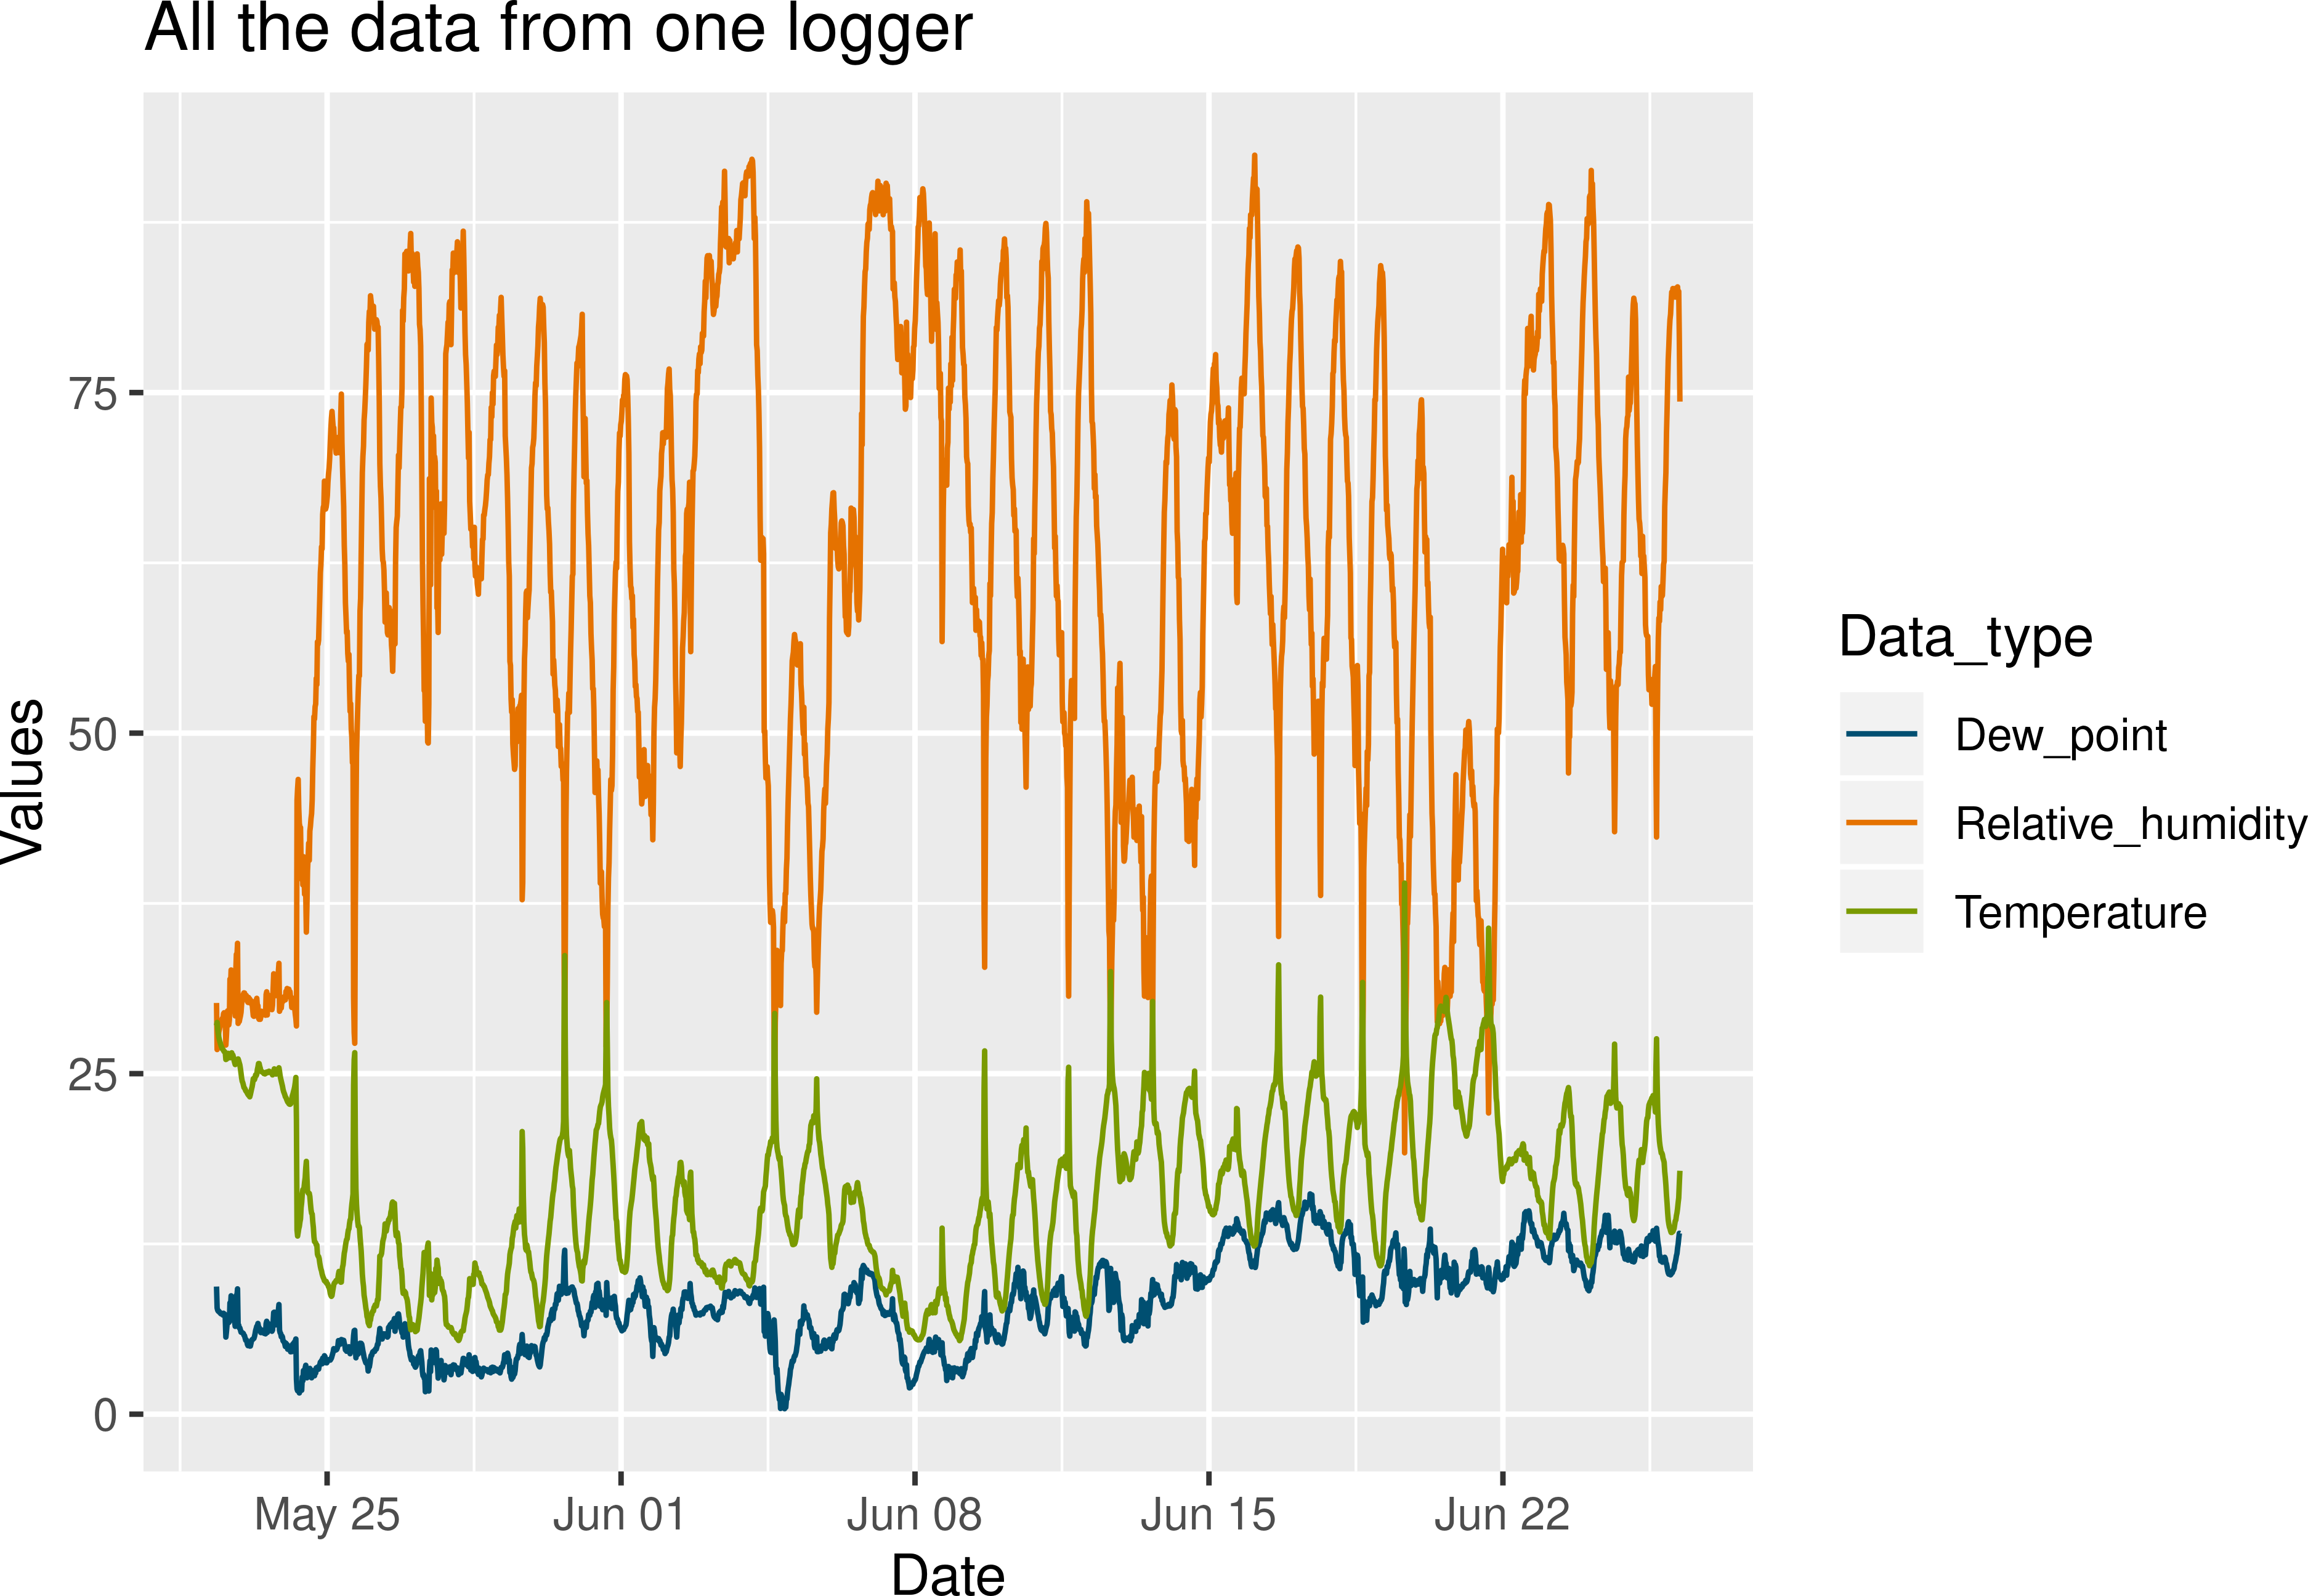
\includegraphics{figure/unnamed-chunk-13-1.png}


\end{document}
